\providecommand{\main}{../../../..}
\documentclass[\main/dresen_thesis.tex]{subfiles}
\begin{document}
  \label{sec:monolayers:nanoparticle:sas}

  By small-angle scattering, the average size and shape of the nanoparticles is probed over a large volume of the sample.
  To evaluate the experimental data quantitatively, a shape model is chosen for a fit to the data.

  \paragraphNewLine{Shape Model}
    In \reffig{fig:monolayers:nanoparticle:sas:AcAcCoFeC} the SAXS data of the nanoparticles synthesized from acetylacetonates is shown.
    The data shows the first form factor minimum at a slightly smaller scattering vector for Ac-CoFe-C in direct comparison and the maxima are also qualitatively sharper for this nanoparticle batch.
    The smaller position of the minima tells that the average particle size is slightly larger for Ac-CoFe-C in comparison to Ac-CoFe-C-2, and the sharper maxima correspond to a smaller size distribution if both particles have a similar shape.

    To obtain a quantitative evaluation of the SAXS data, the parameters are fit to the form factors of varied shapes.
    The sphere form factor is an approximation for a small freely rotating nanoparticle that is simple to calculate and neglects the actual morphology of the particles.
    The cube form factor assumes perfectly shaped cubes with edged corners and the superball form factor allows to vary continuously in between and models a cube with rounded corners.
    Looking at the three shape model fits in \reffig{fig:monolayers:nanoparticle:sas:AcAcCoFeC}, the sphere form factor underestimates the first form factor maxima, while the cube form factor overestimates it in both cases.
    The superball form factor is able to adjust in between and provides thereby best description of the data.

    The parameters of the three fits for both data sets are tabulated in \reftab{tab:monolayers:nanoparticle:saxs:shapeModelStudy}
    The scattering length density of the core is fixed from the results of the XRD (\refsec{sec:monolayers:nanoparticle:xrd}) and EDX (\refsec{sec:monolayers:nanoparticle:edx}) analysis of the nanoparticles.


    \begin{figure}[!htbp]
      \centering
      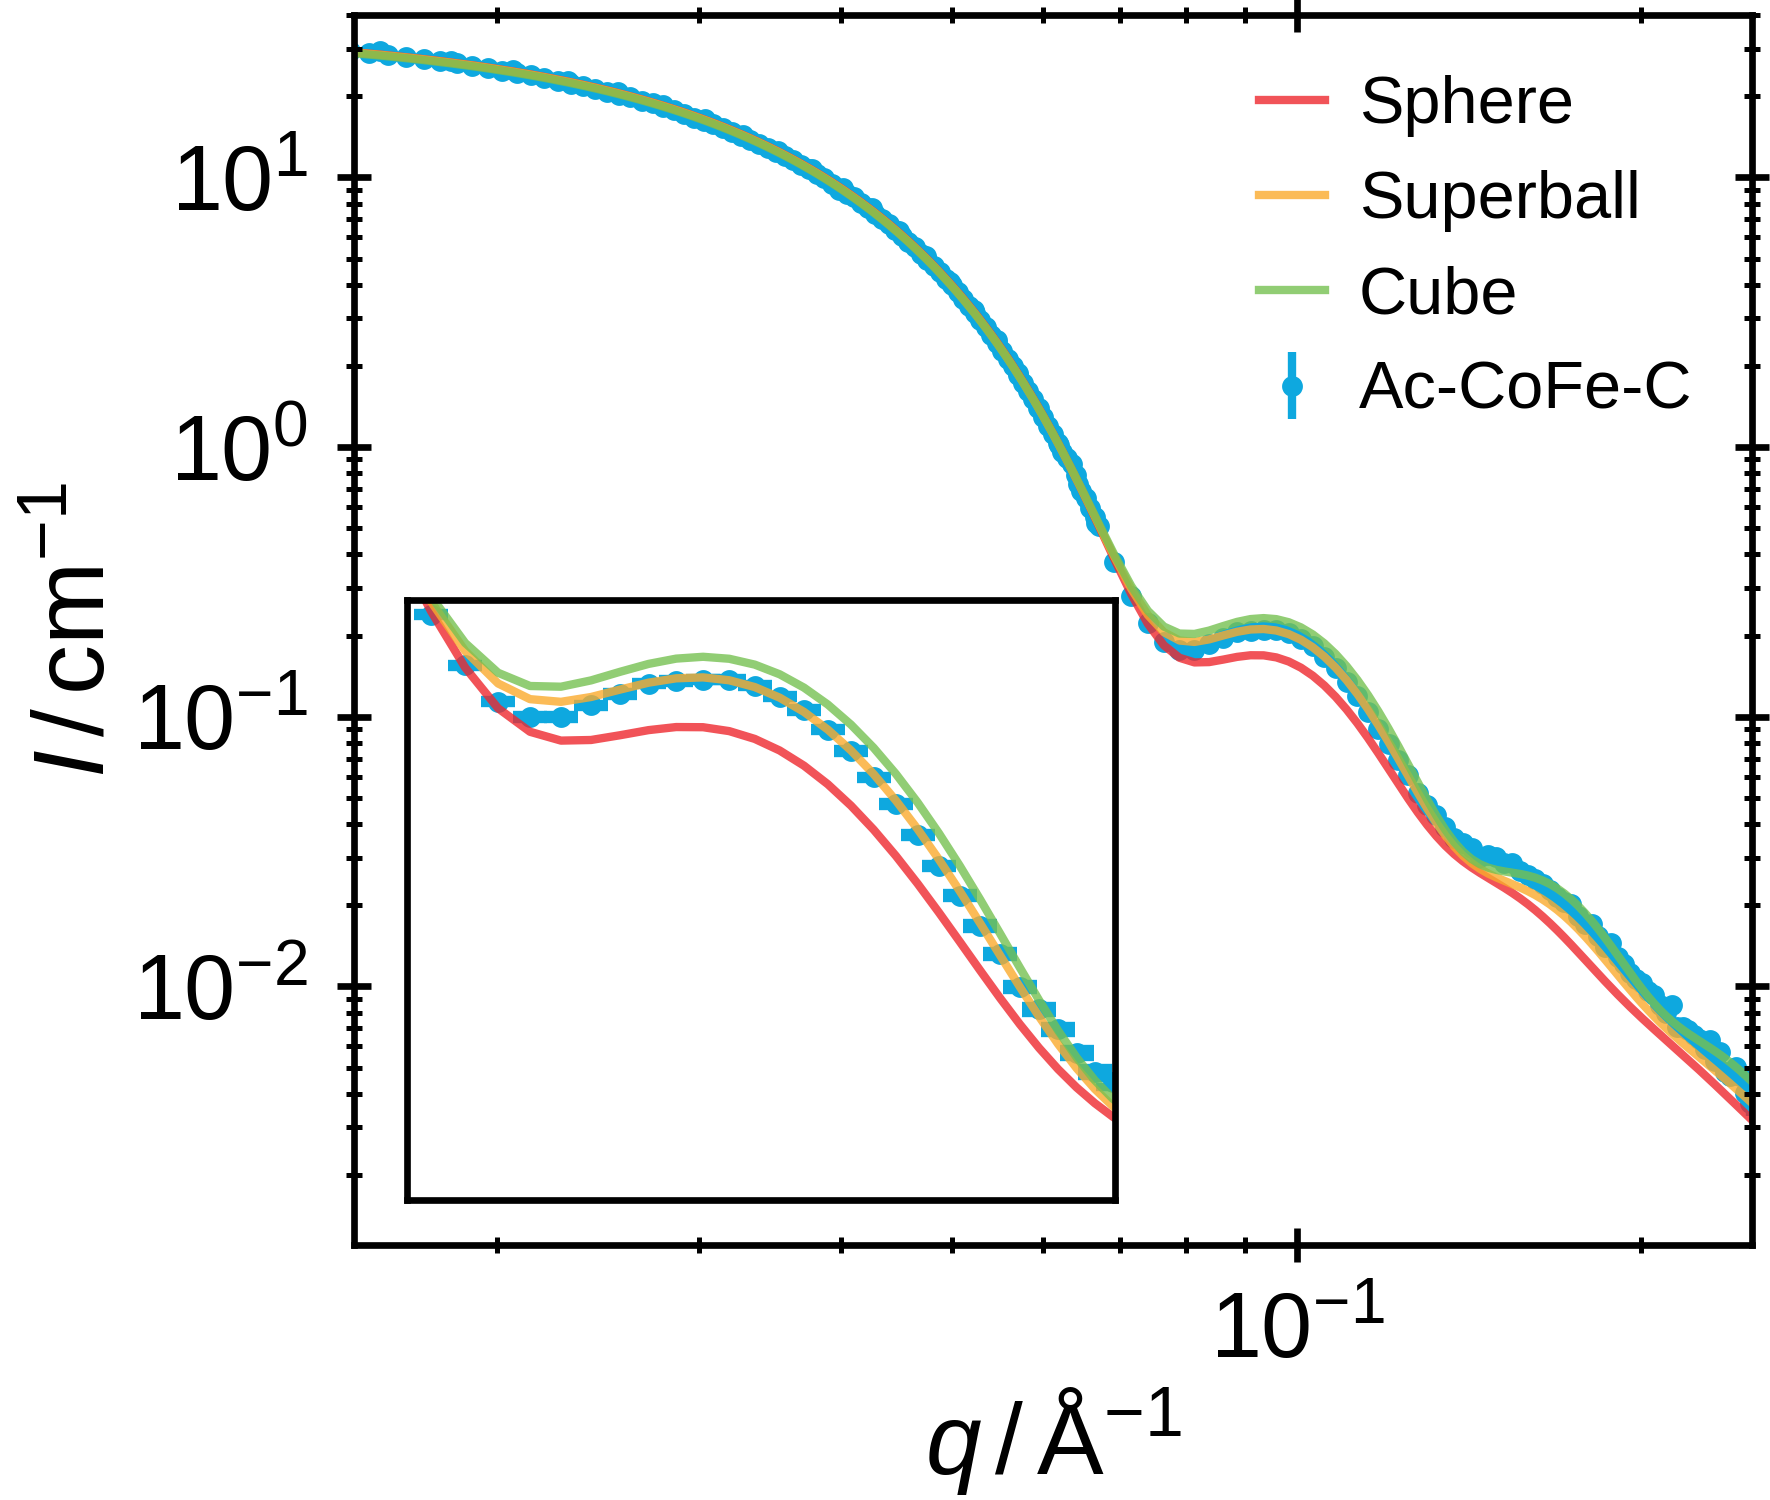
\includegraphics{monolayers_SAS_Ac_CoFe_C_ShapeModelStudy}
      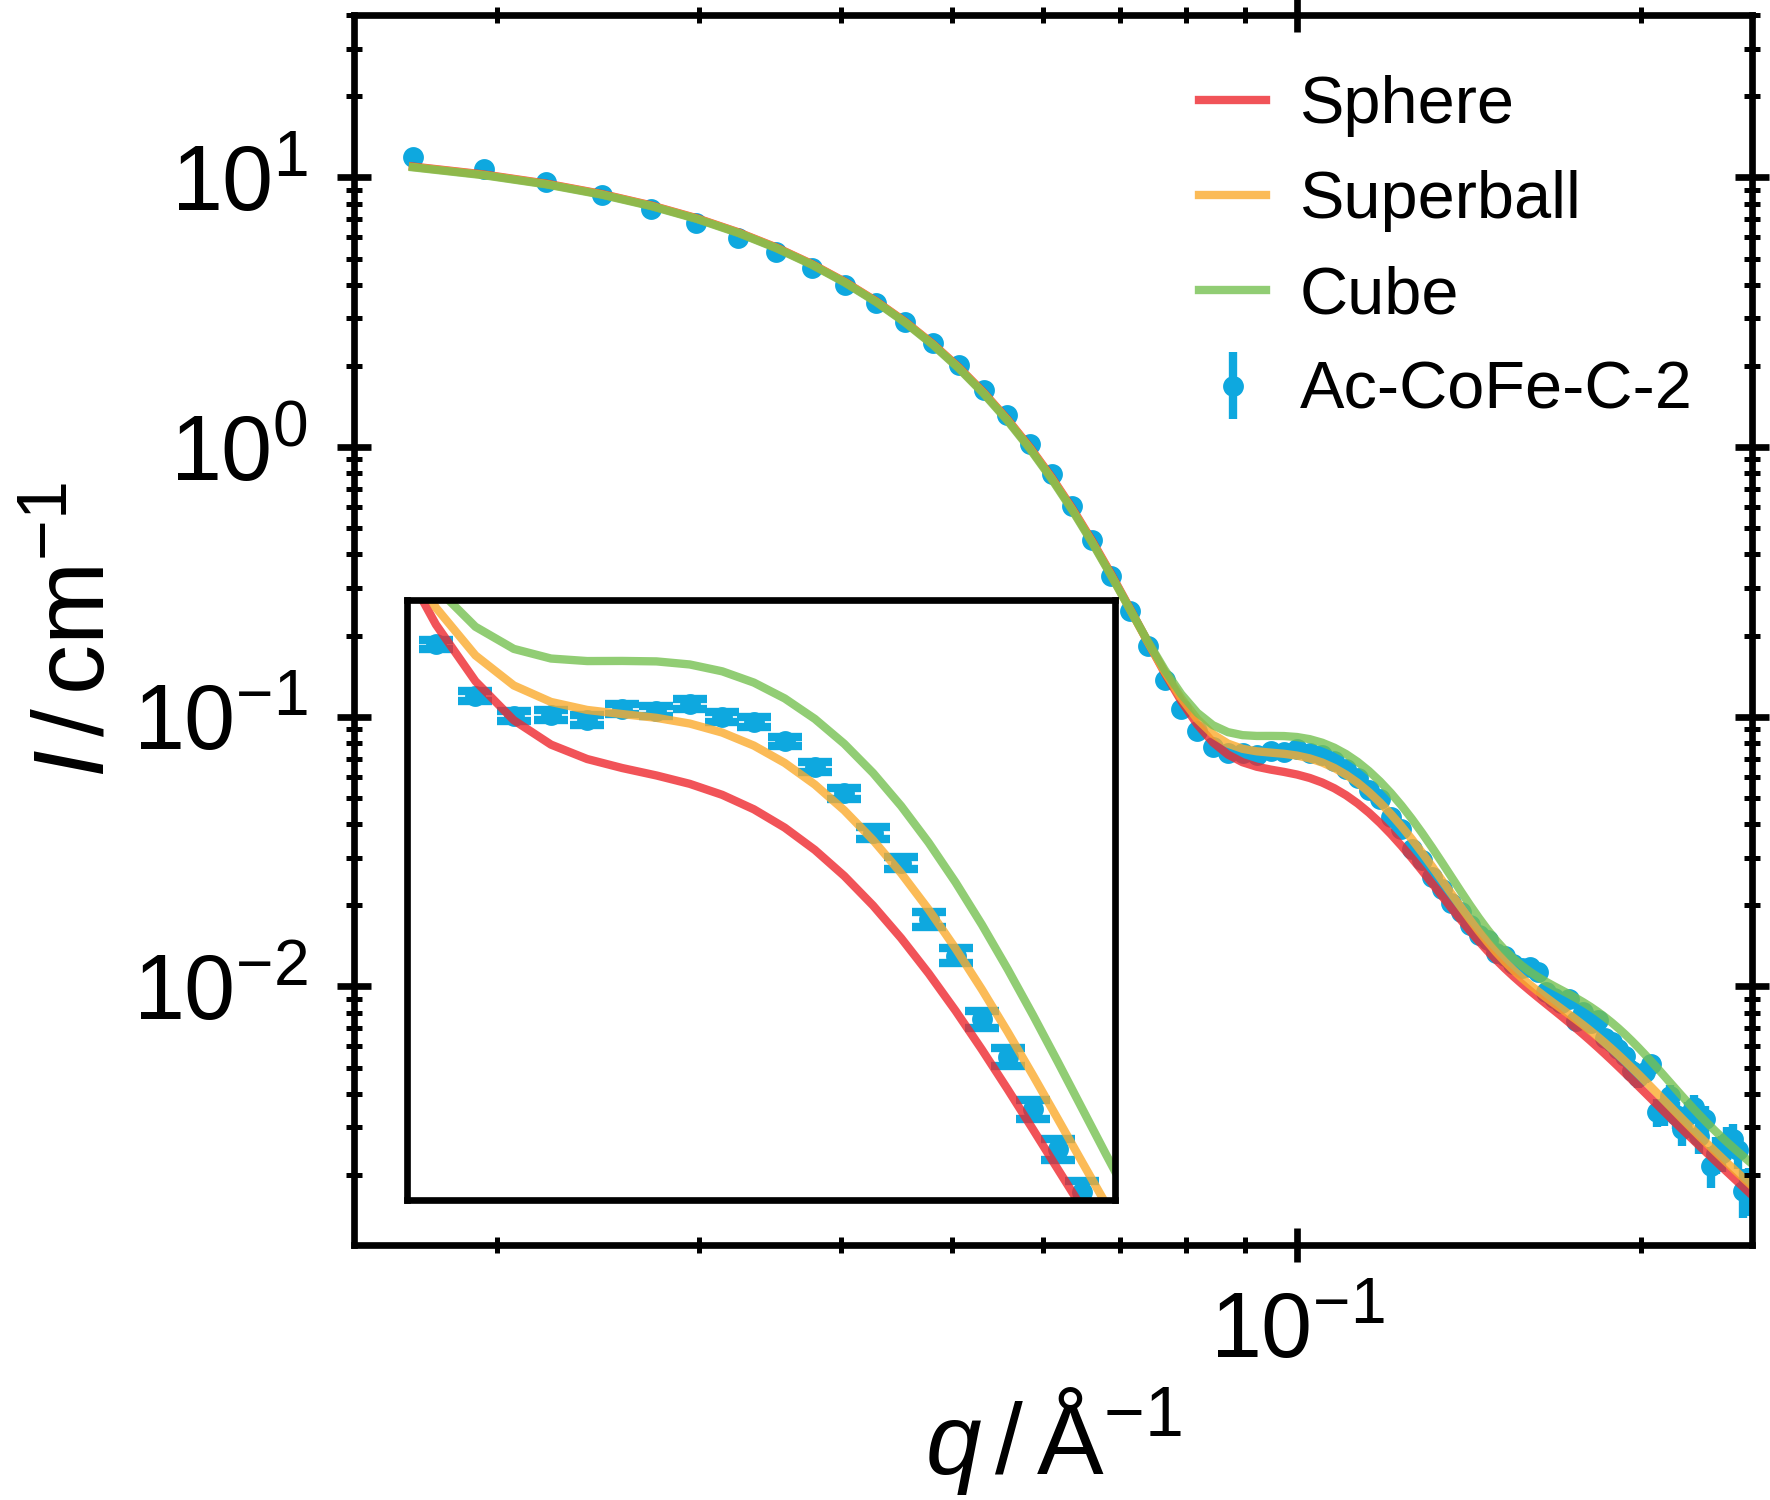
\includegraphics{monolayers_SAS_Ac_CoFe_C_2_ShapeModelStudy}
      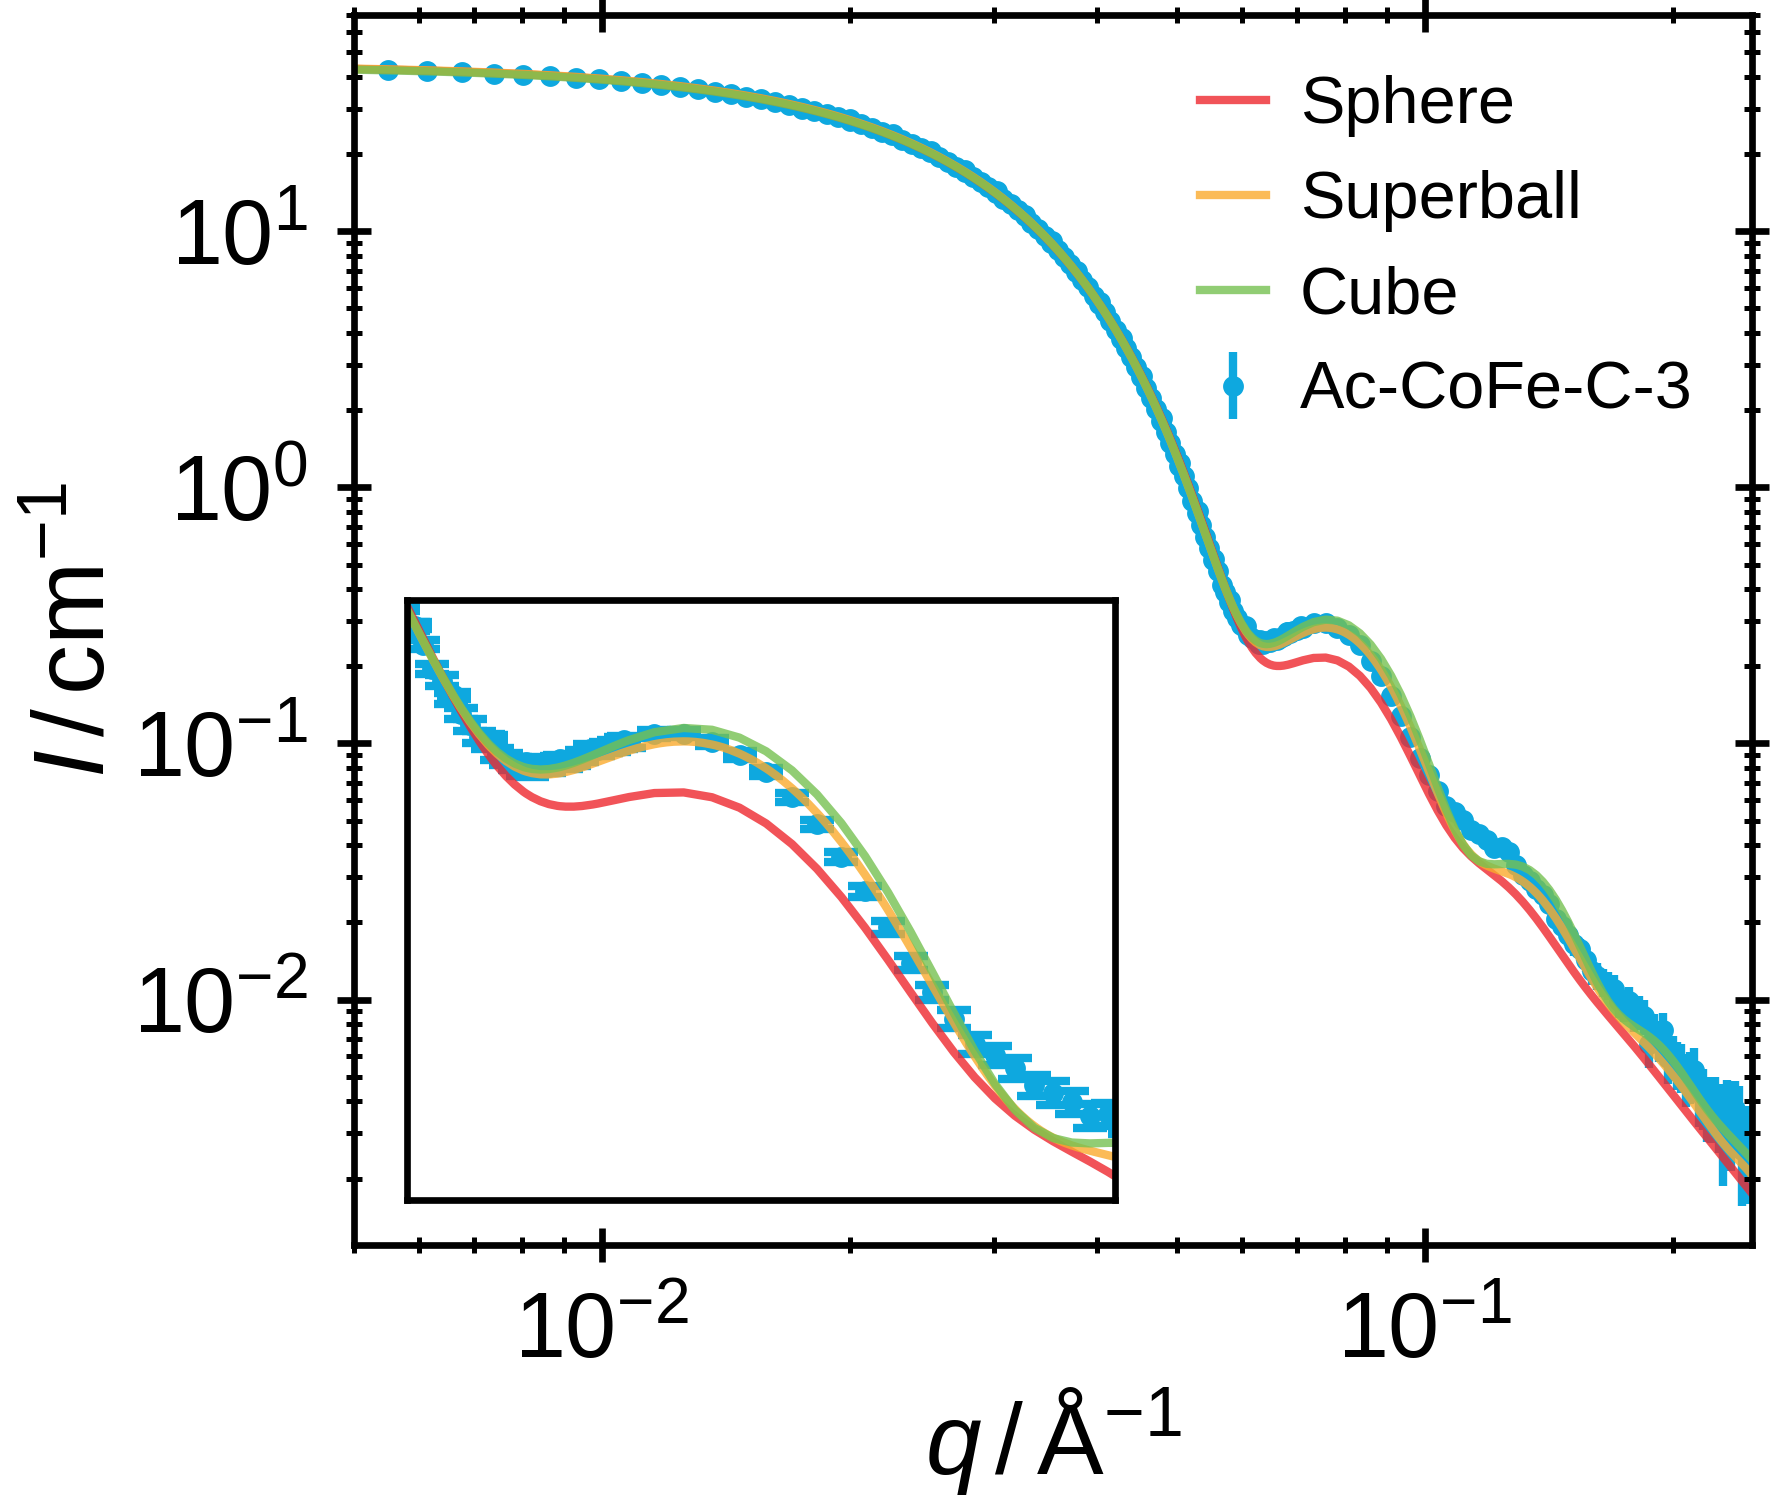
\includegraphics{monolayers_SAS_Ac_CoFe_C_3_ShapeModelStudy}
      \caption{\label{fig:monolayers:nanoparticle:sas:AcAcCoFeC}SAXS data Ac-CoFe-C (upper left), Ac-CoFe-C-2 (upper right) and Ac-CoFe-C-3. In all cases the data is fit to a sphere, cube and superball form factor. The inset zooms to the first form factor maxima.}
    \end{figure}

    \begin{table}[!htbp]
      \centering
      \caption{\label{tab:monolayers:nanoparticle:saxs:shapeModelStudy}Parameters for the form factors of the sphere, cube and superball shown in \reffig{fig:monolayers:nanoparticle:sas:AcAcCoFeC}.
      The size of the sphere and superball are given in terms of the radius $R$, the size of the cube is given in terms of the edge length $a$.
      The respective log-normal size distribution $\sigma_R$ and $\sigma_a$. $n$ is the particle density in dispersion, $p$ the superball exponent and $\rho_\mathrm{core}$, $\rho_\mathrm{solvent}$ the scattering length densities of the particle and the solvent respectively. From the fitted results, the mass concentration $c_m$ is given.}
      \begin{tabular}{ c | l | l | l }
        \textbf{SAXS}  & \textbf{Sphere} & \textbf{Cube} & \textbf{Superball}\\
        \hline
          \multicolumn{4}{l}{\textbf{Ac-CoFe-C}}\\
        \hline
        \rule{0pt}{2ex} $R, \, a \, / \unit{nm}$                      & $5.54(1)$      & $8.97(1)$  & $4.65(2)$\\
        \rule{0pt}{2ex} $\sigma_R, \, \sigma_a \, / \unit{\%}$        & $13.5(2)$      & $11.1(2)$  & $12.3(1)$\\
        \rule{0pt}{2ex} $n \, / 10^{-8} \angstrom^{-3}$               & $0.0420(2)$    & $0.0456(2)$& $0.0439(2)$\\
        \rule{0pt}{2ex} $p$                                           & $1$            & $\infty$   & $2.9(1)$\\
        \hline
        \rule{0pt}{2ex} $\rho_\mathrm{core}    \, / \unit{10^{-6} \angstrom^{-2}}$     & \multicolumn{3}{c}{40.67}\\
        \rule{0pt}{2ex} $\rho_\mathrm{solvent} \, / \unit{10^{-6} \angstrom^{-2}}$     & \multicolumn{3}{c}{6.46}\\
        \hline
        \rule{0pt}{2ex} $c_m \, / \unit{mg\, mL^{-1}}$                & $1.56(2)$      & $1.70(2)$  & $1.63(2)$\\
        \hline
        \rule{0pt}{2ex} $\chi^2$                                      & $120.0$        & $51.8$     & $31.6$\\
        \hline
        \hline
        \multicolumn{4}{l}{\textbf{Ac-CoFe-C-2}}\\
        \hline
        \rule{0pt}{2ex} $R, \, a \, / \unit{nm}$                      & $4.98(2)$      & $8.10(4)$  & $4.29(4)$\\
        \rule{0pt}{2ex} $\sigma_R \, / \unit{\%}$                     & $15.9(4)$      & $13.6(4)$  & $15.0(4)$\\
        \rule{0pt}{2ex} $n \, / 10^{-8} \angstrom^{-3}$               & $0.0287(3)$    & $0.0307(4)$& $0.0293(3)$\\
        \rule{0pt}{2ex} $p$                                           & $1$            & $\infty$   & $2.2(2)$\\
        \hline
        \rule{0pt}{2ex} $\rho_\mathrm{core}    \, / \unit{10^{-6} \angstrom^{-2}}$     & \multicolumn{3}{c}{41.21}\\
        \rule{0pt}{2ex} $\rho_\mathrm{solvent} \, / \unit{10^{-6} \angstrom^{-2}}$     & \multicolumn{3}{c}{8.01}\\
        \hline
        \rule{0pt}{2ex} $c_m \, / \unit{mg\, mL^{-1}}$                & $0.77(1)$      & $0.84(2)$  & $0.80(2)$\\
        \hline
        \rule{0pt}{2ex} $\chi^2$                                      & $69.4$         & $70.8$     & $51.9$\\
        \hline
        \hline
        \multicolumn{4}{l}{\textbf{Ac-CoFe-C-3}}\\
        \hline
        \rule{0pt}{2ex} $R, \, a \, / \unit{nm}$                      & $68.6(2)$      & $11.2(1)$  & $5.69(2)$\\
        \rule{0pt}{2ex} $\sigma_R \, / \unit{\%}$                     & $13.4(2)$      & $10.5(1)$  & $11.0(1)$\\
        \rule{0pt}{2ex} $n \, / 10^{-8} \angstrom^{-3}$               & $0.0153(1)$    & $0.0165(1)$& $0.0161(1)$\\
        \rule{0pt}{2ex} $p$                                           & $1$            & $\infty$   & $4.1(3)$\\
        \hline
        \rule{0pt}{2ex} $\rho_\mathrm{core}    \, / \unit{10^{-6} \angstrom^{-2}}$     & \multicolumn{3}{c}{41.97}\\
        \rule{0pt}{2ex} $\rho_\mathrm{solvent} \, / \unit{10^{-6} \angstrom^{-2}}$     & \multicolumn{3}{c}{8.01}\\
        \hline
        \rule{0pt}{2ex} $c_m \, / \unit{mg\, mL^{-1}}$                & $1.09(1)$      & $1.19(2)$  & $1.15(2))$\\
        \hline
        \rule{0pt}{2ex} $\chi^2$                                      & $17.8$         & $3.5$     & $2.9$\\
        \hline
      \end{tabular}
    \end{table}

  \paragraphNewLine{SANS Model: Oleic Acid Shell and Micelles}
    The SANS data of Ac-CoFe-C and Ac-CoFe-C-2 in \reffig{fig:monolayers:nanoparticle:sans:superballAcAcFit} reveals the first two form factor maxima, and in total three minima can be seen in both cases.
    The fitted model is a sum of two form factors, one from a superball with an oleic acid shell, and the other a spherical formfactor to model oleic acid micelles in the dispersion.
    The varied parameters are tabulated in \reftab{tab:monolayers:nanoparticle:sans:superballAcAcFit}, where the particle dimension, size distribution and superball exponent are set to the values from SAXS in \reftab{tab:monolayers:nanoparticle:saxs:shapeModelStudy}.
    The inset of \reffig{fig:monolayers:nanoparticle:sans:superballAcAcFit} shows the scattering length density profiles to visualize the length scales of the core and shell size.
    For the superball the shown SLD profile represents a cut along one of the four fold axes.

    \begin{figure}[!htbp]
      \centering
      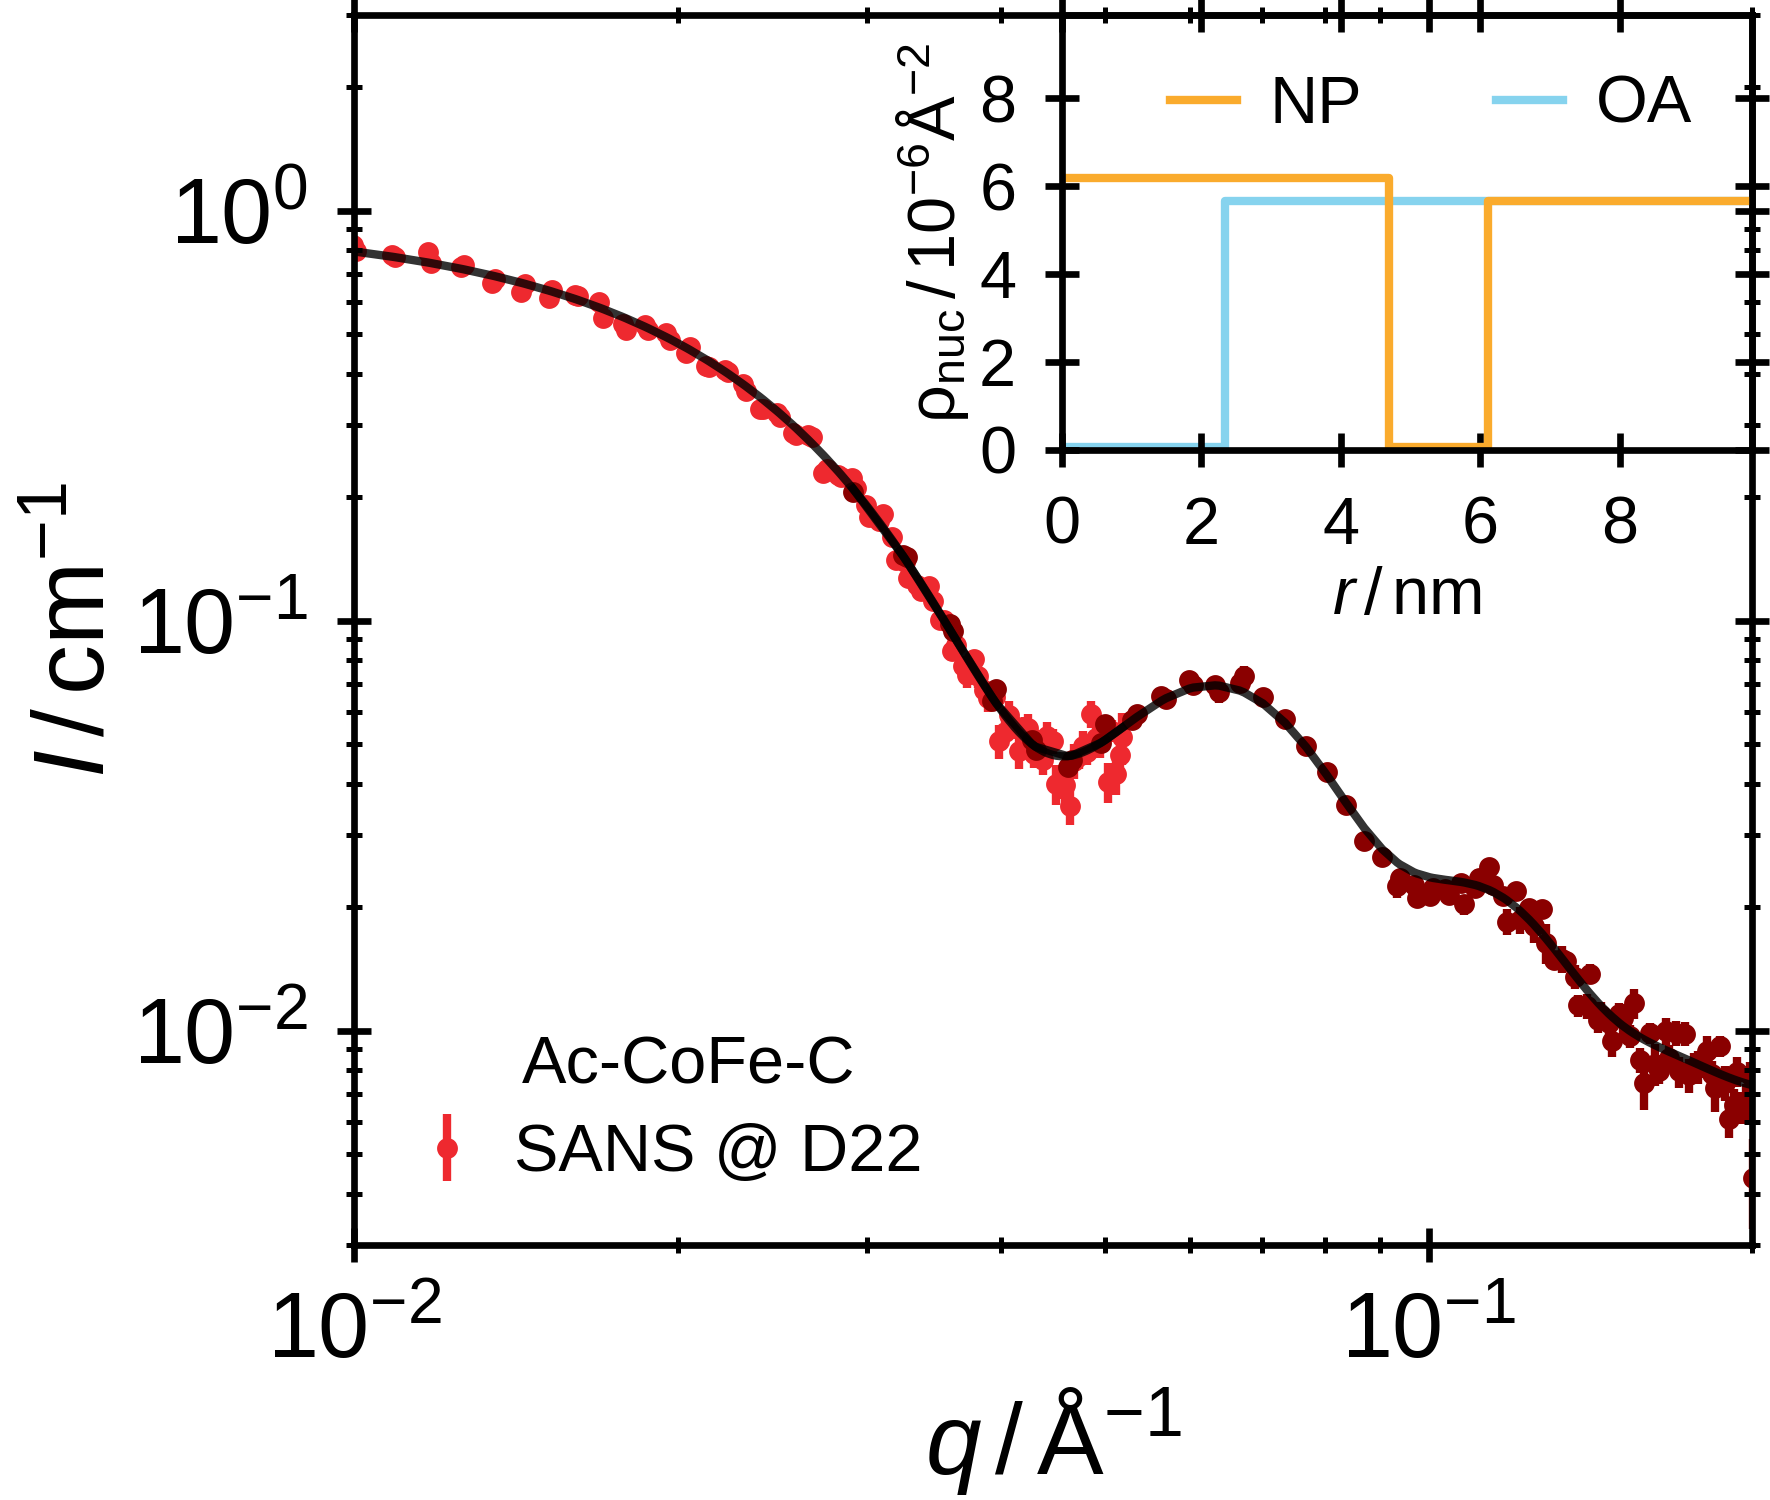
\includegraphics{monolayers_SAS_Ac_CoFe_C_SANS}
      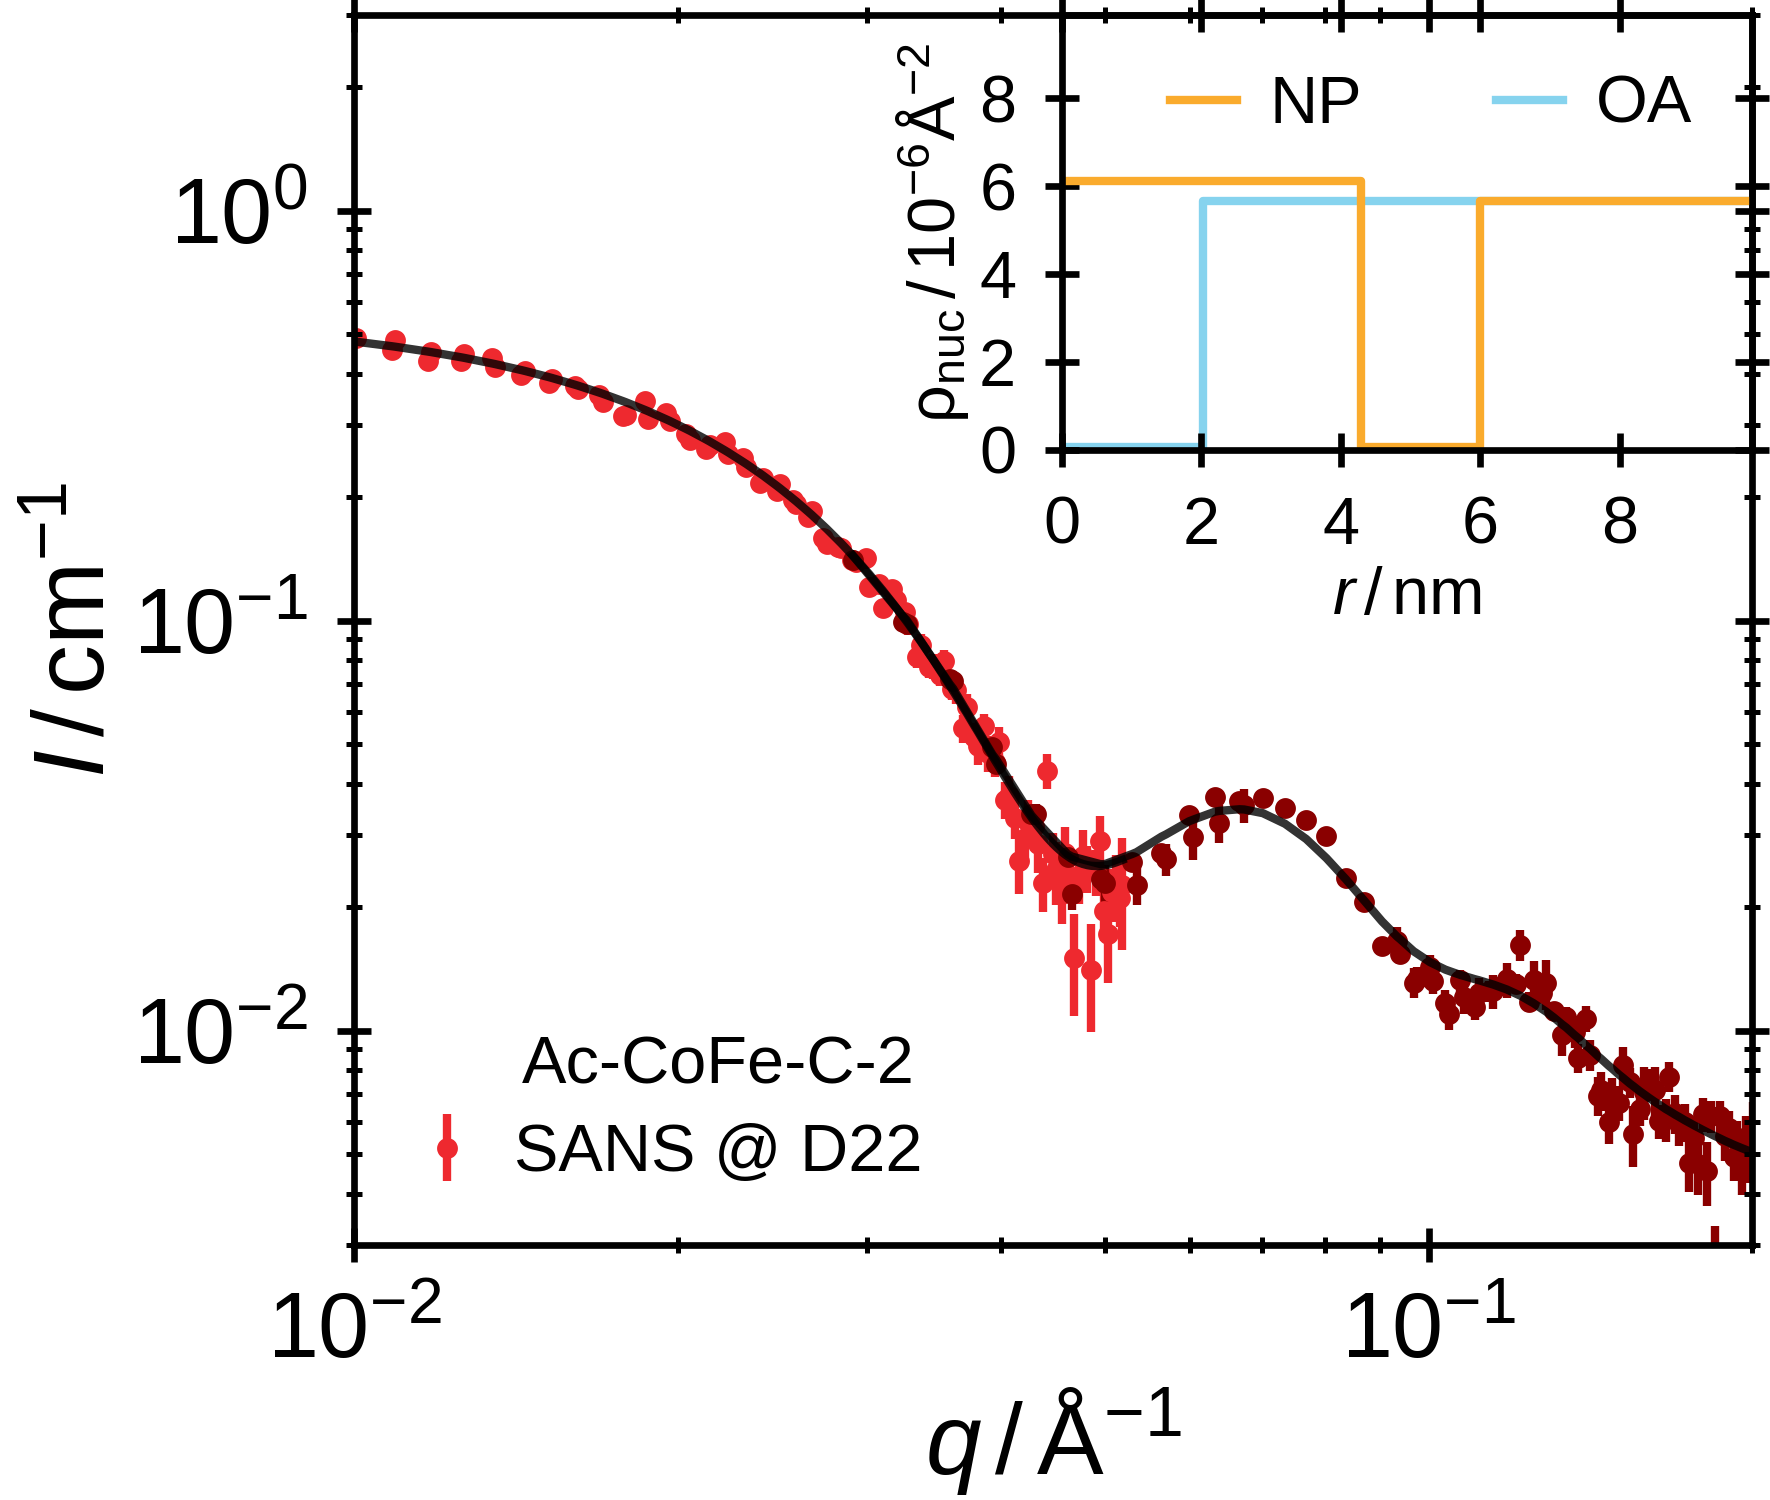
\includegraphics{monolayers_SAS_Ac_CoFe_C_2_SANS}
      \caption{\label{fig:monolayers:nanoparticle:sans:superballAcAcFit}Ac-CoFe-C (left) and Ac-CoFe-C-2 (right) SANS data described by the sum of a superball form factor and a spherical form factor. The inset shows the SLD profiles of the superball nanoparticles (orange line) and the spherical oleic acid micelles (blue line) for the SANS data. The parameters of the form factors are listed in \reftab{tab:monolayers:nanoparticle:sans:superballAcAcFit}.}
    \end{figure}

    \begin{figure}[!htbp]
      \centering
      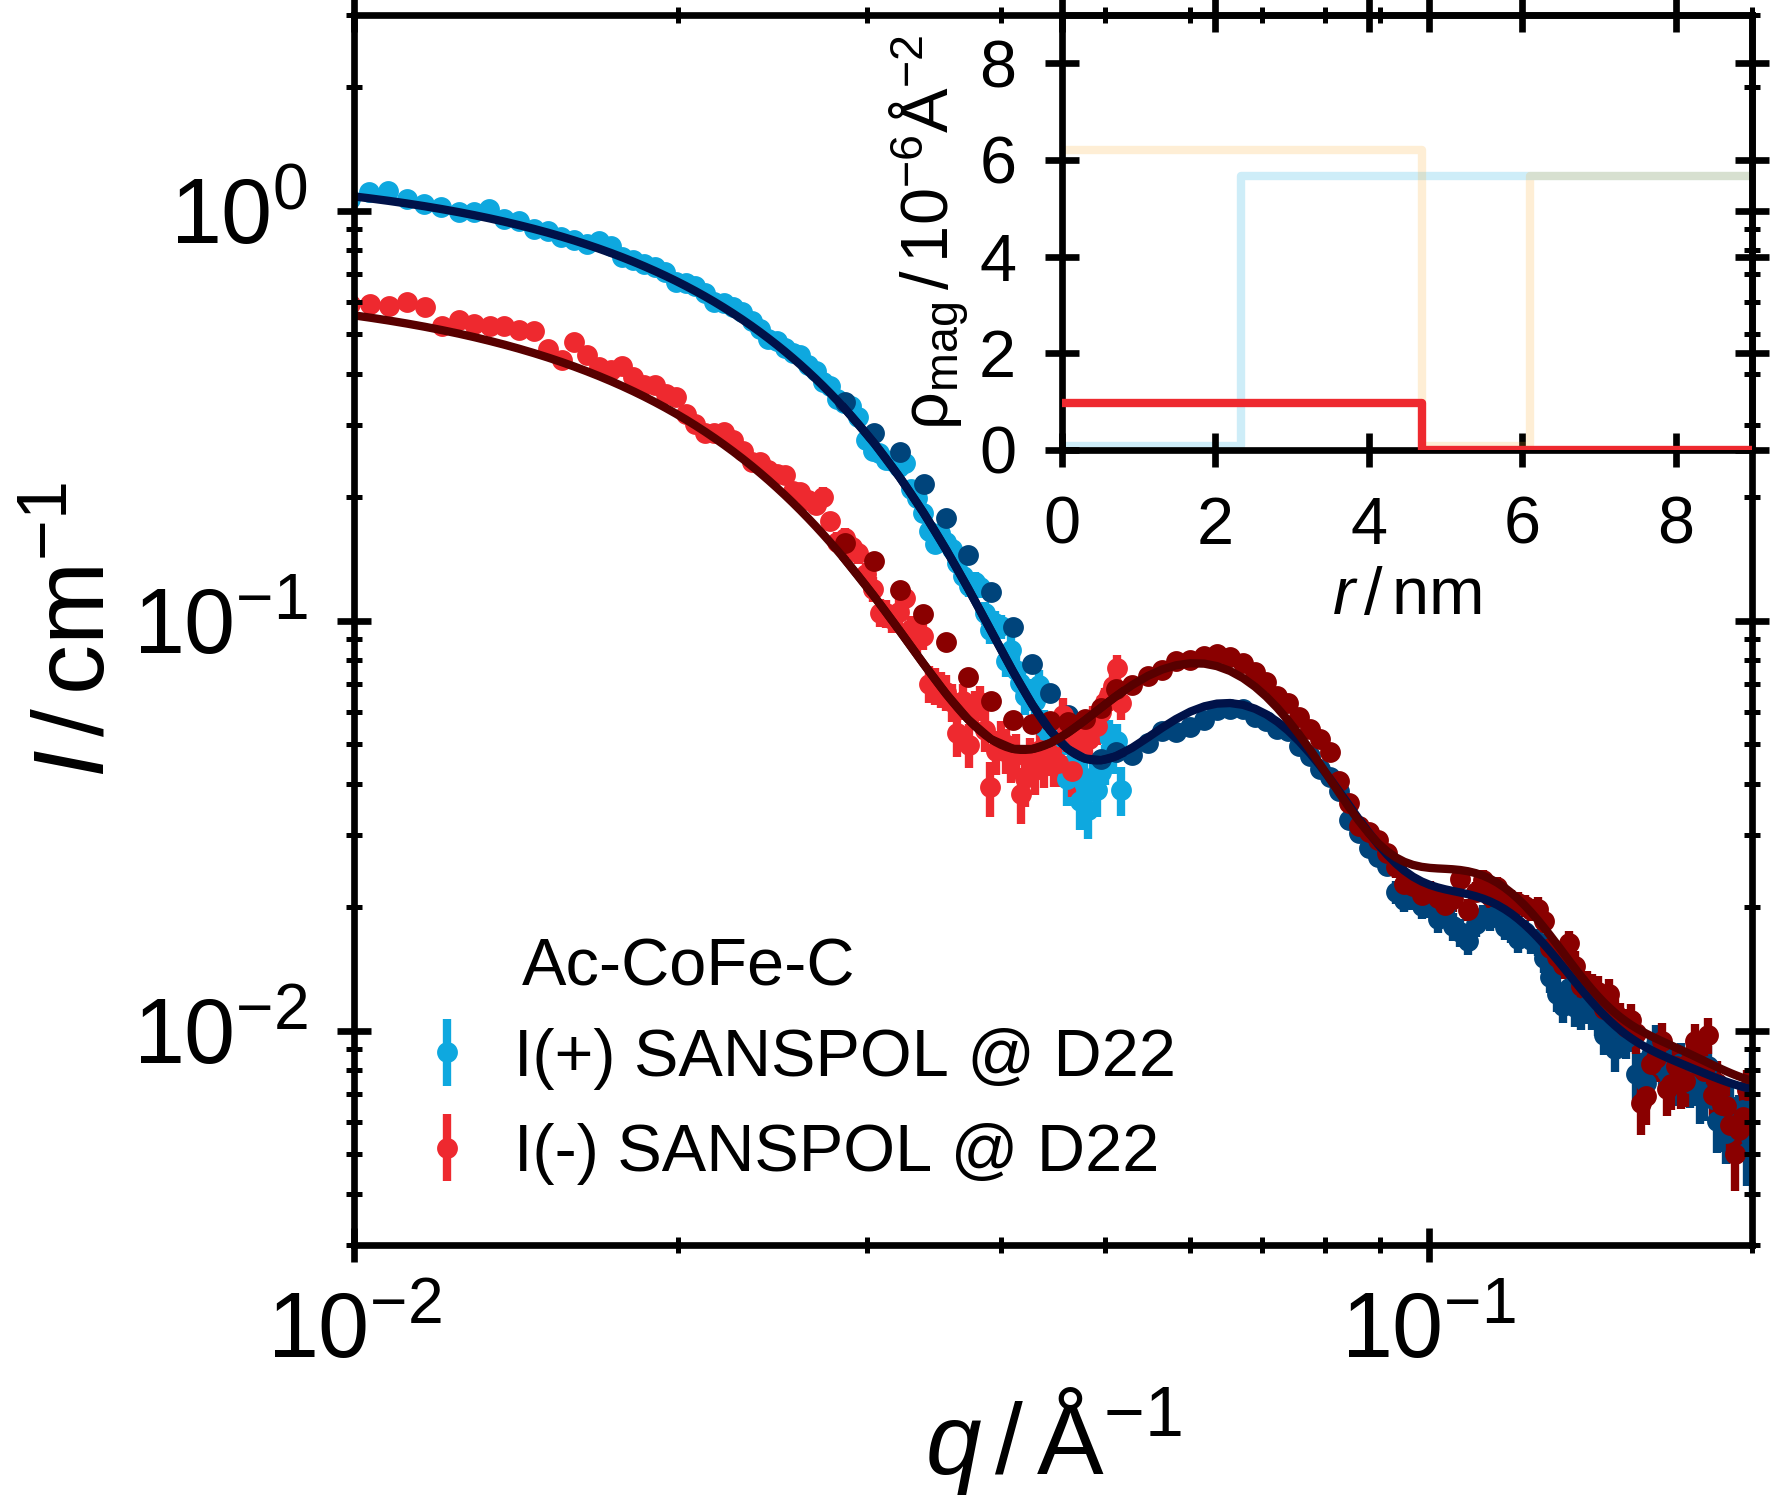
\includegraphics{monolayers_SAS_Ac_CoFe_C_SANSPOLFit}
      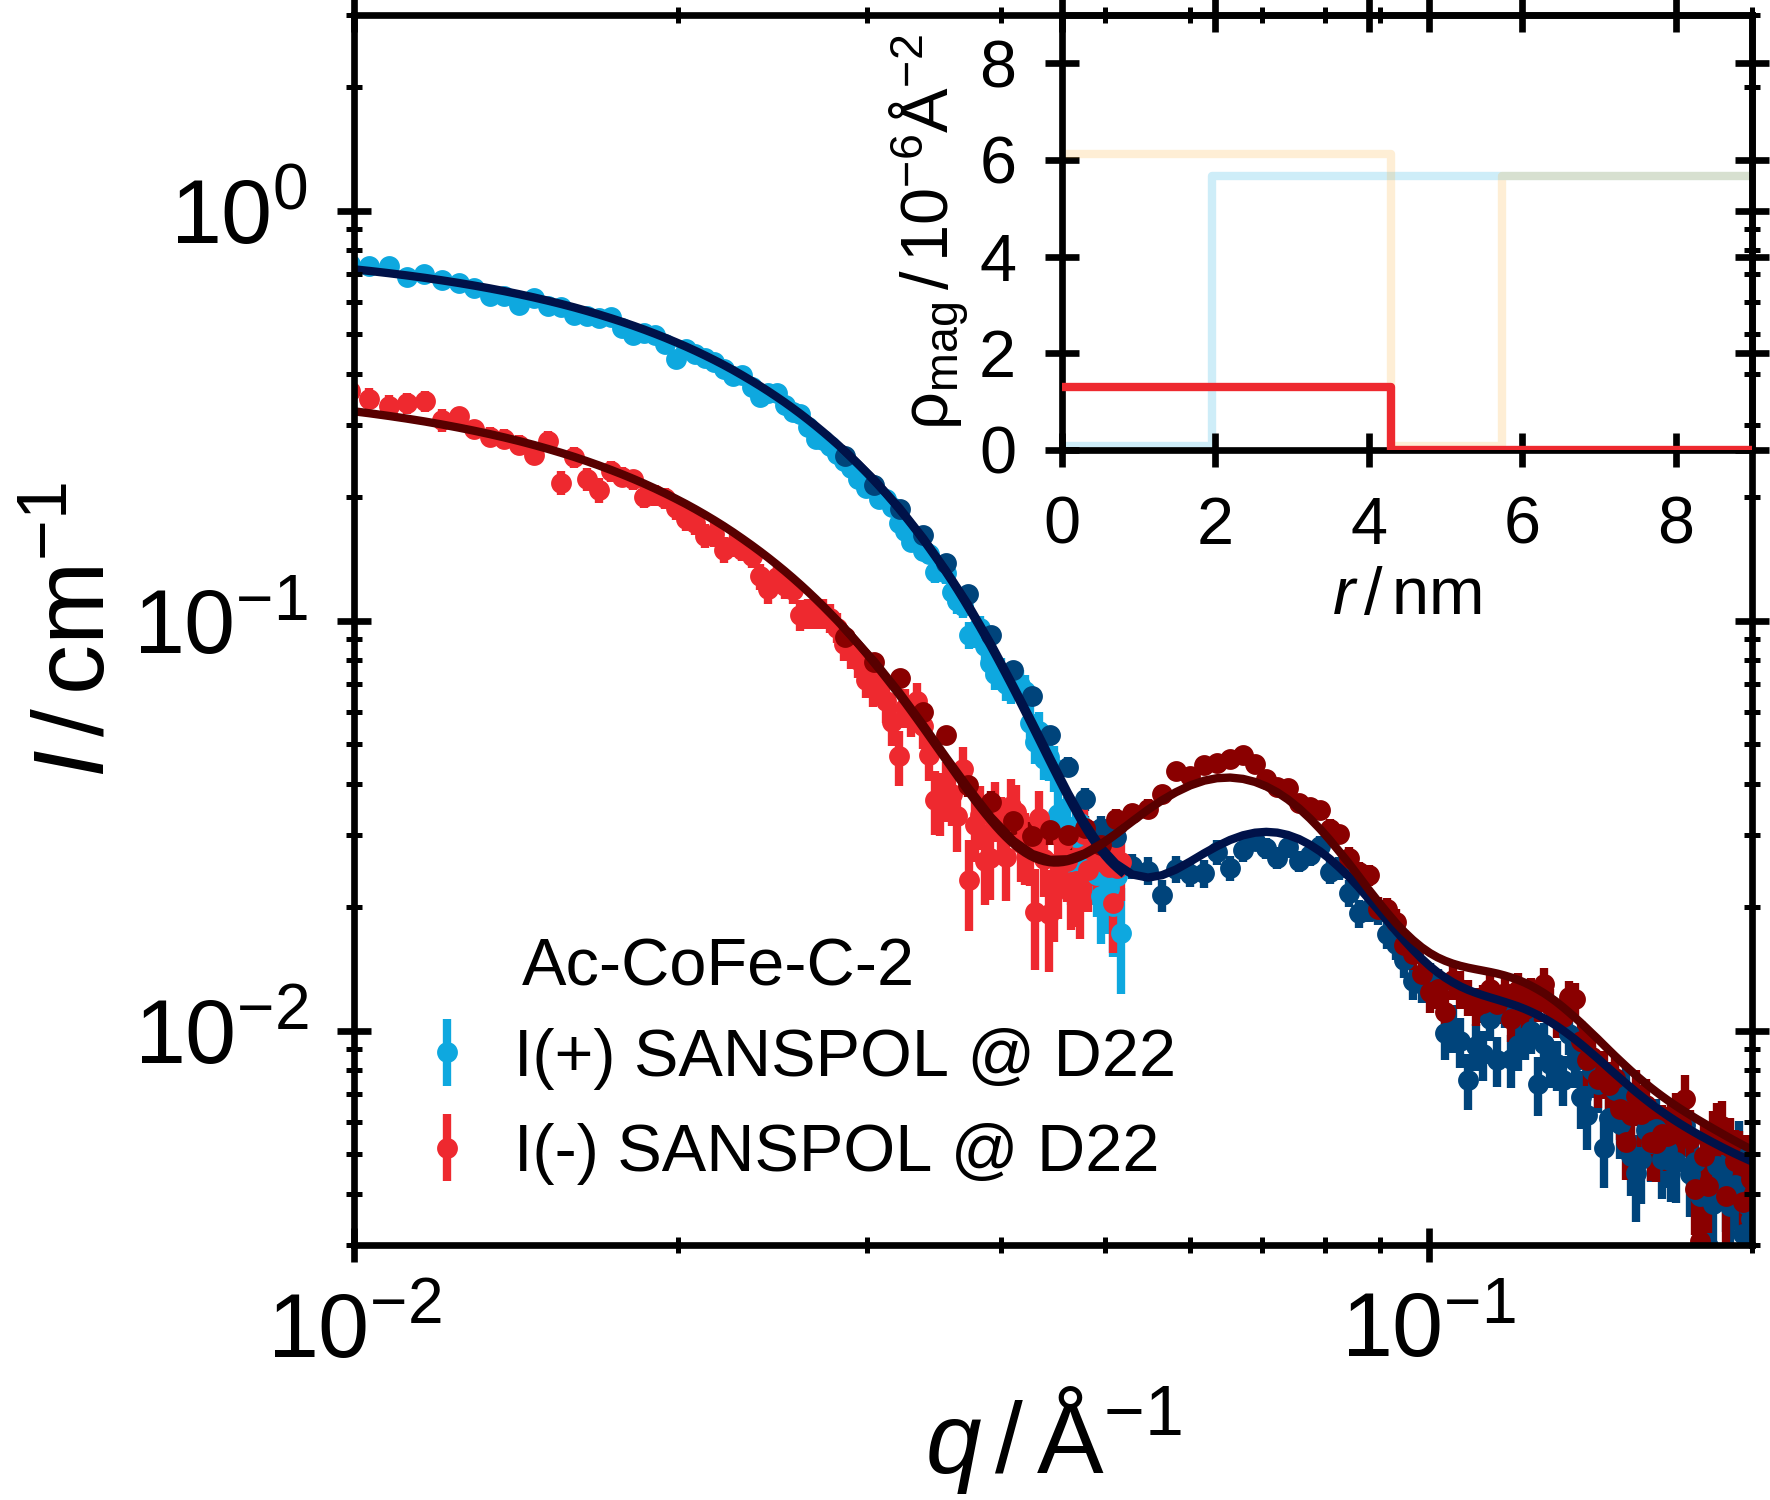
\includegraphics{monolayers_SAS_Ac_CoFe_C_2_SANSPOLFit}
      \caption{\label{fig:monolayers:nanoparticle:sanspol:superballAcAcFit}SANSPOL data of Ac-CoFe-C (left) and Ac-CoFe-C-2 (right) fit with the same nuclear form factor as in \reffig{fig:monolayers:nanoparticle:sans:superballAcAcFit} to determine the magnetic scattering length density  shown in the inset (red line). The parameters are listed in \reftab{tab:monolayers:nanoparticle:sans:superballAcAcFit}.}
    \end{figure}

    \begin{table}[!htbp]
      \centering
      \caption{\label{tab:monolayers:nanoparticle:sans:superballAcAcFit}Parameters for the Ac-CoFe-C and Ac-CoFe-C-2 SANS superball formfactor and oleic acid micelles background shown in \reffig{fig:monolayers:nanoparticle:sas:AcAcCoFeC}.
      The size, size-distribution and exponent of the superball are used as in \reftab{tab:monolayers:nanoparticle:saxs:shapeModelStudy}.
      The nuclear SLD of the particle $\rho_\mathrm{core}$, oleic acid shell $\rho_\mathrm{OA}$ and solvent $\rho_\mathrm{solvent}$ are given, as well as the constant background $I_\mathrm{bg}$. From the size and number density $n$, the mass concentration $c_m$ of the particles and volume fraction $c_V$ of oleic acid are calculated. From SANSPOL the magnetic SLD $\rho_\mathrm{mag}$ and thereby the magnetization $M$ are given.}
      \begin{tabular}{ c | l | l }
        \textbf{SANS}  & \textbf{Ac-CoFe-C} & \textbf{Ac-CoFe-C-2}\\
        \hline
        \rule{0pt}{2ex} $d / \unit{nm}$                                              & $1.41(3)$      & $1.41$  \\
        \rule{0pt}{2ex} $r_\mathrm{OA} / \unit{nm}$                                  & $2.34(3)$      & $2.0(1)$  \\
        \rule{0pt}{2ex} $n_\mathrm{NP} \, / \unit{10^{-8} \angstrom^{-3}}$                  & $0.041(2)$     & $0.0334(3)$ \\
        \rule{0pt}{2ex} $n_\mathrm{OA} \, / \unit{10^{-8} \angstrom^{-3}}$                  & $0.43(3)$      & $0.46(13)$  \\
        \hline
        \rule{0pt}{2ex} $\rho_\mathrm{core}    \, / \unit{10^{-6} \angstrom^{-2}}$   & $6.198$        & $6.132$    \\
        \hline
        \rule{0pt}{2ex} $\rho_\mathrm{OA}      \, / \unit{10^{-6} \angstrom^{-2}}$   & \multicolumn{2}{c}{0.078}\\
        \rule{0pt}{2ex} $\rho_\mathrm{solvent} \, / \unit{10^{-6} \angstrom^{-2}}$   & \multicolumn{2}{c}{5.664}\\
        \hline
        \rule{0pt}{2ex} $I_\mathrm{bg} \, / \unit{cm^{-1}}$                          & $0.0061(2)$    & $0.0039(4)$\\
        \hline
        \rule{0pt}{2ex} $c_{m, \, \mathrm{NP}} \, / \unit{mg\, mL^{-1}}$             & $1.5(1)$       & $1.25(1)$  \\
        \rule{0pt}{2ex} $c_{V, \, \mathrm{OA}} \, / \unit{10^{-3}}$                  & $0.23(2)$      & $0.14(1)$  \\
        \hline
        \rule{0pt}{2ex} $\chi^2$                                                     & $2.0$          & $2.6$      \\
        \hline
        \textbf{SANSPOL}\\
        \hline
        \rule{0pt}{2ex} $\rho_\mathrm{mag} \, / \unit{10^{-6} \angstrom^{-2}}$       & $0.97(2)$      & $1.29(1)$  \\
        \rule{0pt}{2ex} $M \, / \unit{kA \,m^{-1}}$                                  & $334(5)$       & $444(3)$   \\
        \hline
        \rule{0pt}{2ex} $\chi^2$                                                     & $4.4$          & $1.7$      \\
      \end{tabular}
    \end{table}

    The best fit shows a good agreement with the shell thickness of $1.41 \unit{nm}$ for Ac-CoFe-C and $1.70 \unit{nm}$ for Ac-CoFe-C-2.
    The average micelles radius is estimated to $2.34 \unit{nm}$ and $2.02 \unit{nm}$ respectively.
    The volume fraction of the oleic acid micelles is in both cases in the order of $c_V \eq 2 \cdot 10^{-4}$, meaning that in $10 \unit{mL}$ of dispersion, $2 \unit{\musf L}$ of additional oleic acid is found.

    In \cite{Disch_2010_Thesp}, it is estimated that the head-to-tail distance of oleic acid is $2.1 \unit{nm}$.
    The determined size for the micelles is in a similar order of magnitude, whereas the size for the nanoparticle shell thickness is slightly lower.
    The slight variation of the micelle size can be explained to an insufficient signal-to-noise ratio to properly determine the micelle size from the background to high precision.
    The deviation for the nanoparticle shell might be explained due to either an deviation of the superball shape for the oleic acid shell or an intermixing of the oleic acid shell with the solvent.
    Both effects are modeled effectively by a reduced shell thickness, as the oleic acid SLD is fixed to the literature bulk value.

    The determined mass concentration for the Ac-CoFe-C nanoparticles is $1.5(1) \unit{mg\, mL^{-1}}$, which is in agreement with the SAXS value of $1.63(2) \unit{mg\, mL^{-1}}$.
    For Ac-CoFe-C-2 the mass concentration is $0.58(4) \unit{mg\, mL^{-1}}$, which is also in a similar order as the SAXS result of $0.80(2) \unit{mg \, mL^{-1}}$.
    The deviation is possible as the SANS dispersions were redispersed for the measurement from the stock solution.

  \paragraphNewLine{Core-Shell Form Factor for Ol-CoFe-C}
    \begin{table}[!htbp]
      \centering
      \caption{\label{tab:monolayers:nanoparticle:sans:superballOlFit}Fit parameters of the core-shell superball model used to describe Ol-CoFe-C.
      Given are the radius of the core $R_\textsf{w\"ustite}$, the thickness of the shell $d_\mathrm{inv.\,spinell}$, the thickness of the oleic acid shell $d_\mathrm{OA}$, as well as the log-normal particle size distribution $\sigma_{R+d}$, the particle number density $n$ and the superball exponent $p$. The fitted core and shell composition as well as the scattering length densities $\rho$ are stated. Additionally a background of oleic acid micelles with radius $r_\mathrm{OA}$ and number density $n_\mathrm{OA}$ is fitted.
      The mass concentration $c_m$ of the core-shell nanoparticles and $c_V$ of oleic acid are determined. From SANSPOL the magnetic SLD $\rho_\mathrm{mag}$ and from this the magnetization $M$ is determined.}
      \begin{tabular}{ c | l | l }
        \textbf{SAS} & \multicolumn{2}{c}{\textbf{Ol-CoFe-C}}\\
        \hline
                     & \textbf{SAXS} & \textbf{SANS}\\
        \hline
        \rule{0pt}{2ex} $R_\textsf{w\"ustite} \, / \unit{nm}$                        & \multicolumn{2}{c}{$1.7(1)$}\\
        \rule{0pt}{2ex} $d_\mathrm{inv.\,spinell} / \unit{nm}$                       & \multicolumn{2}{c}{$3.4(1)$}\\
        \rule{0pt}{2ex} $\sigma_{R+d} \, / \unit{\%}$                                & \multicolumn{2}{c}{$6.2(3)$}\\
        \rule{0pt}{2ex} $\sigma_{d} \, / \unit{\%}$                                  & \multicolumn{2}{c}{$18(4)$}\\
        \rule{0pt}{2ex} $d_\mathrm{OA} / \unit{nm}$                                  & \multicolumn{2}{c}{$1.58(4)$}\\
        \rule{0pt}{2ex} $p$                                                          & \multicolumn{2}{c}{$4.1(4)$ }\\
        \hline
        \rule{0pt}{2ex} Core                                                         & \multicolumn{2}{c}{\ch{Fe_{0.48(1)} Co_{0.52(1)} O}}\\
        \rule{0pt}{2ex} Shell                                                        & \multicolumn{2}{c}{\ch{Co_{0.82(1)} Fe_{2.18(1)} O_4}}\\
        \hline
        \rule{0pt}{2ex} $n \, / 10^{-8} \angstrom^{-3}$                              & $0.0300(3)$     & $0.130(7)$\\
        \hline
        \rule{0pt}{2ex} $\rho_\mathrm{core}    \, / \unit{10^{-6} \angstrom^{-2}}$   & $51(1)$  & $6.2(1)$\\
        \rule{0pt}{2ex} $\rho_\mathrm{shell}   \, / \unit{10^{-6} \angstrom^{-2}}$   & $41(1)$  & $6.1(1)$\\
        \rule{0pt}{2ex} $\rho_\mathrm{OA}      \, / \unit{10^{-6} \angstrom^{-2}}$   & $8.52$   & $0.078$\\
        \rule{0pt}{2ex} $\rho_\mathrm{solvent} \, / \unit{10^{-6} \angstrom^{-2}}$   & $7.55$   & $5.664$\\
        \rule{0pt}{2ex} $I_\mathrm{bg} \, / \unit{cm^{-1}}$                          & $0$      & $0.130(7)$\\
        \hline
        \rule{0pt}{2ex} $n_\mathrm{OA} \, / 10^{-8} \angstrom^{-3}$                  & \multicolumn{2}{c}{$0.69(8)$}\\
        \rule{0pt}{2ex} $r_\mathrm{OA} / \unit{nm}$                                  & \multicolumn{2}{c}{$2.1$}\\
        \hline
        \rule{0pt}{2ex} $c_{m, \, \mathrm{NP}} \, / \unit{mg\, mL^{-1}}$             & $1.6(1)$  & $6.9(1)$\\
        \rule{0pt}{2ex} $c_{V, \, \mathrm{OA}} \, / \unit{10^{-3}}$                  & \multicolumn{2}{c}{$0.24(1)$}\\
        \hline
        \rule{0pt}{2ex} $\chi^2$                                                     & $46$     & $3.6$\\
        \hline
        \textbf{SANSPOL}\\
        \hline
        \rule{0pt}{2ex} $\rho_\mathrm{mag}^\mathrm{core} \, / \unit{10^{-6} \angstrom^{-2}}$ & \multicolumn{2}{c}{$0.00(1)$}\\
        \rule{0pt}{2ex} $\rho_\mathrm{mag}^\mathrm{shell} \, / \unit{10^{-6} \angstrom^{-2}}$& \multicolumn{2}{c}{$0.33(3)$}\\
        \rule{0pt}{2ex} $M_\mathrm{core} \, / \unit{kA \,m^{-1}}$                    & \multicolumn{2}{c}{$0(3)$}\\
        \rule{0pt}{2ex} $M_\mathrm{shell} \, / \unit{kA \,m^{-1}}$                   & \multicolumn{2}{c}{$113(12)$}\\
        \hline
        \rule{0pt}{2ex} $\chi^2$                                                     & \multicolumn{2}{c}{$1.75$}\\
      \end{tabular}
    \end{table}


    \begin{figure}[tb]
      \centering
      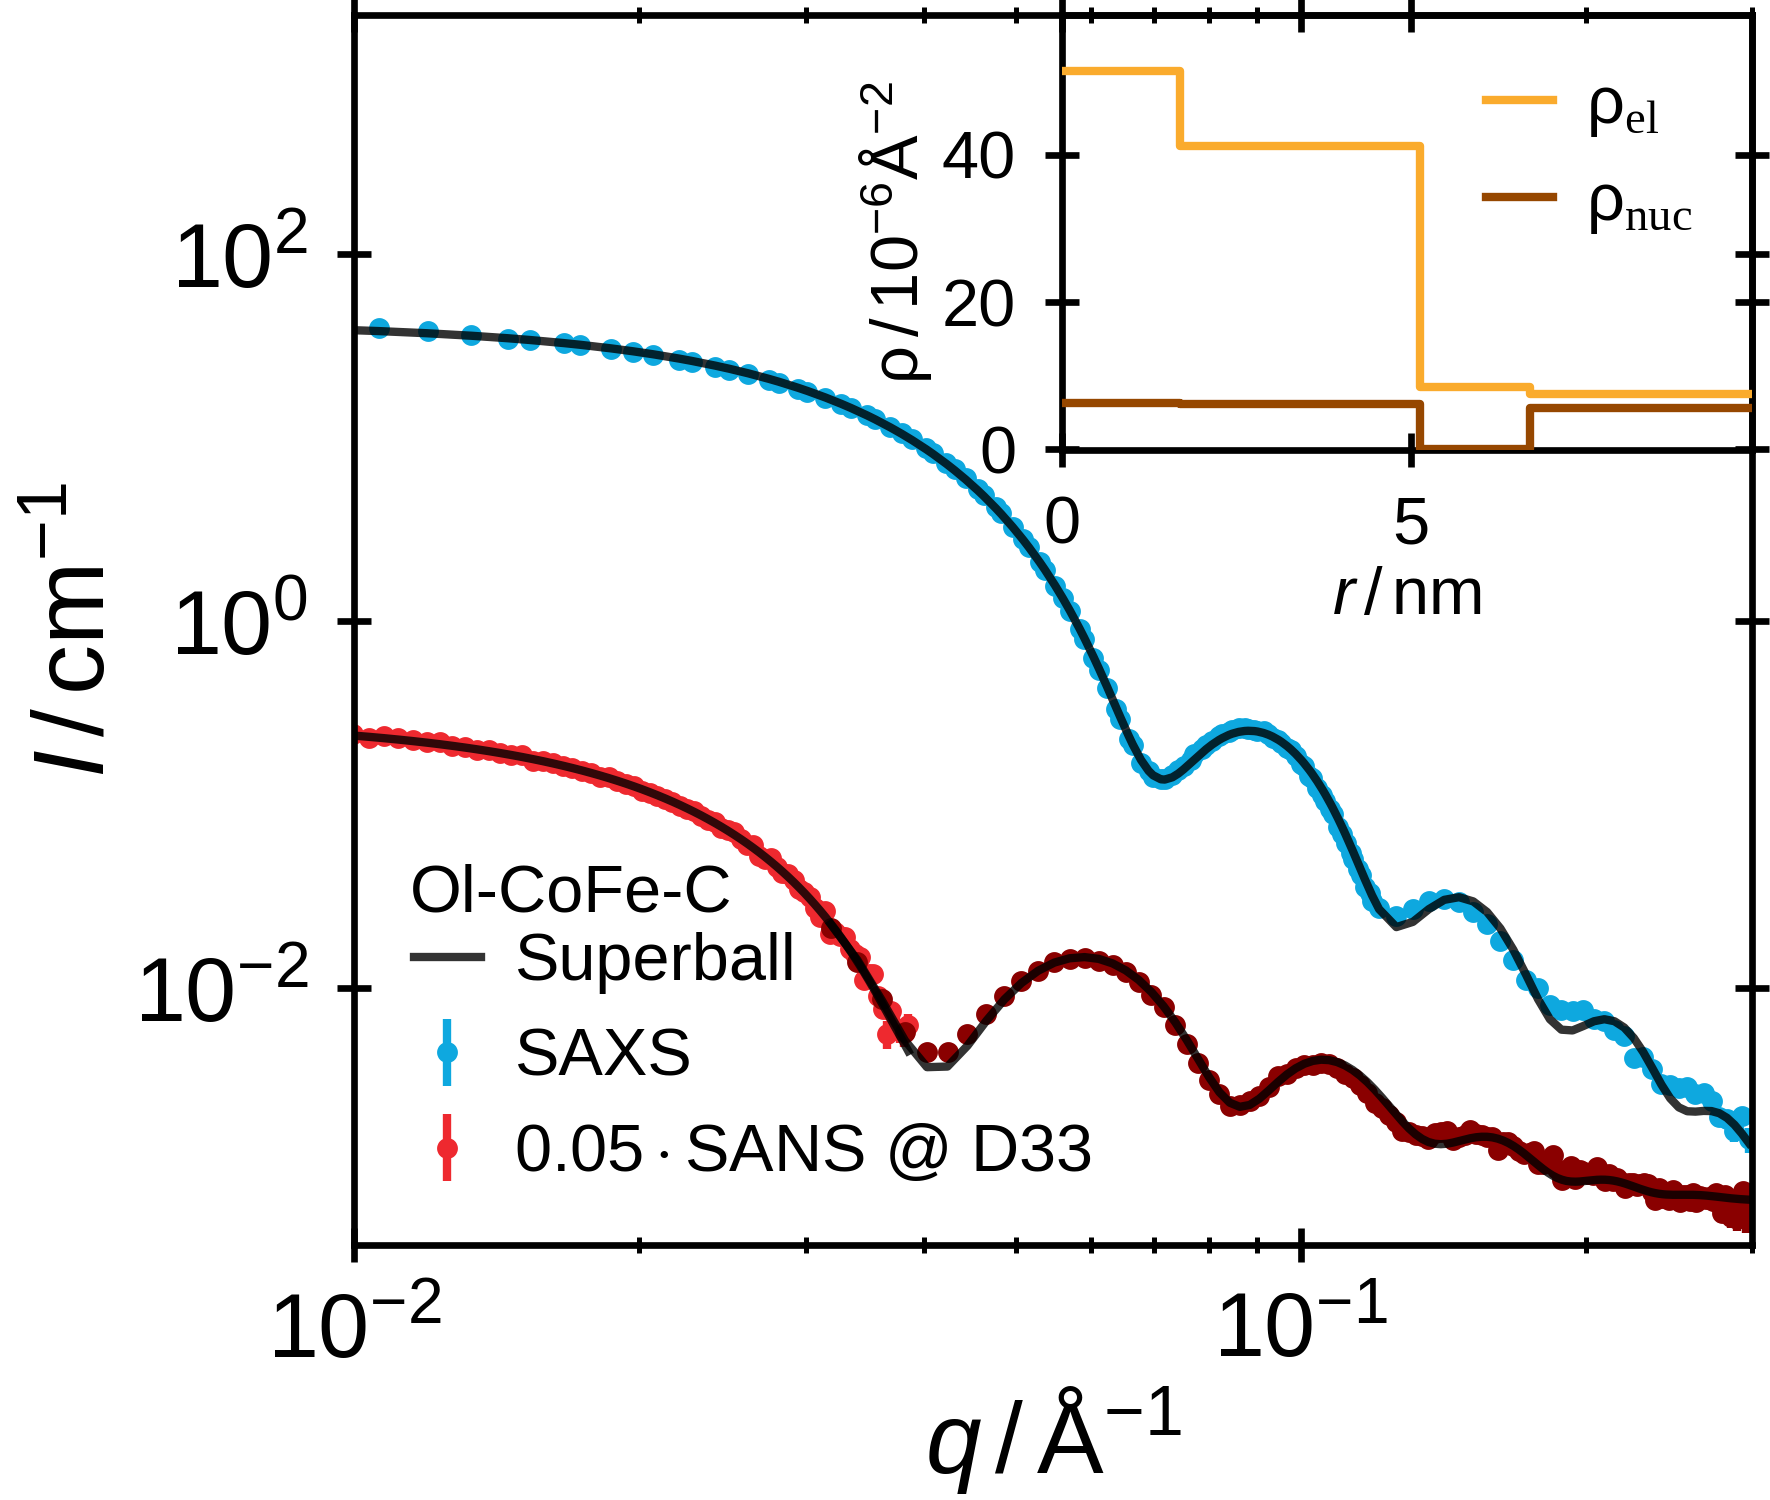
\includegraphics{monolayers_SAS_Ol_CoFe_C_SimultaneousSaxsSans}
      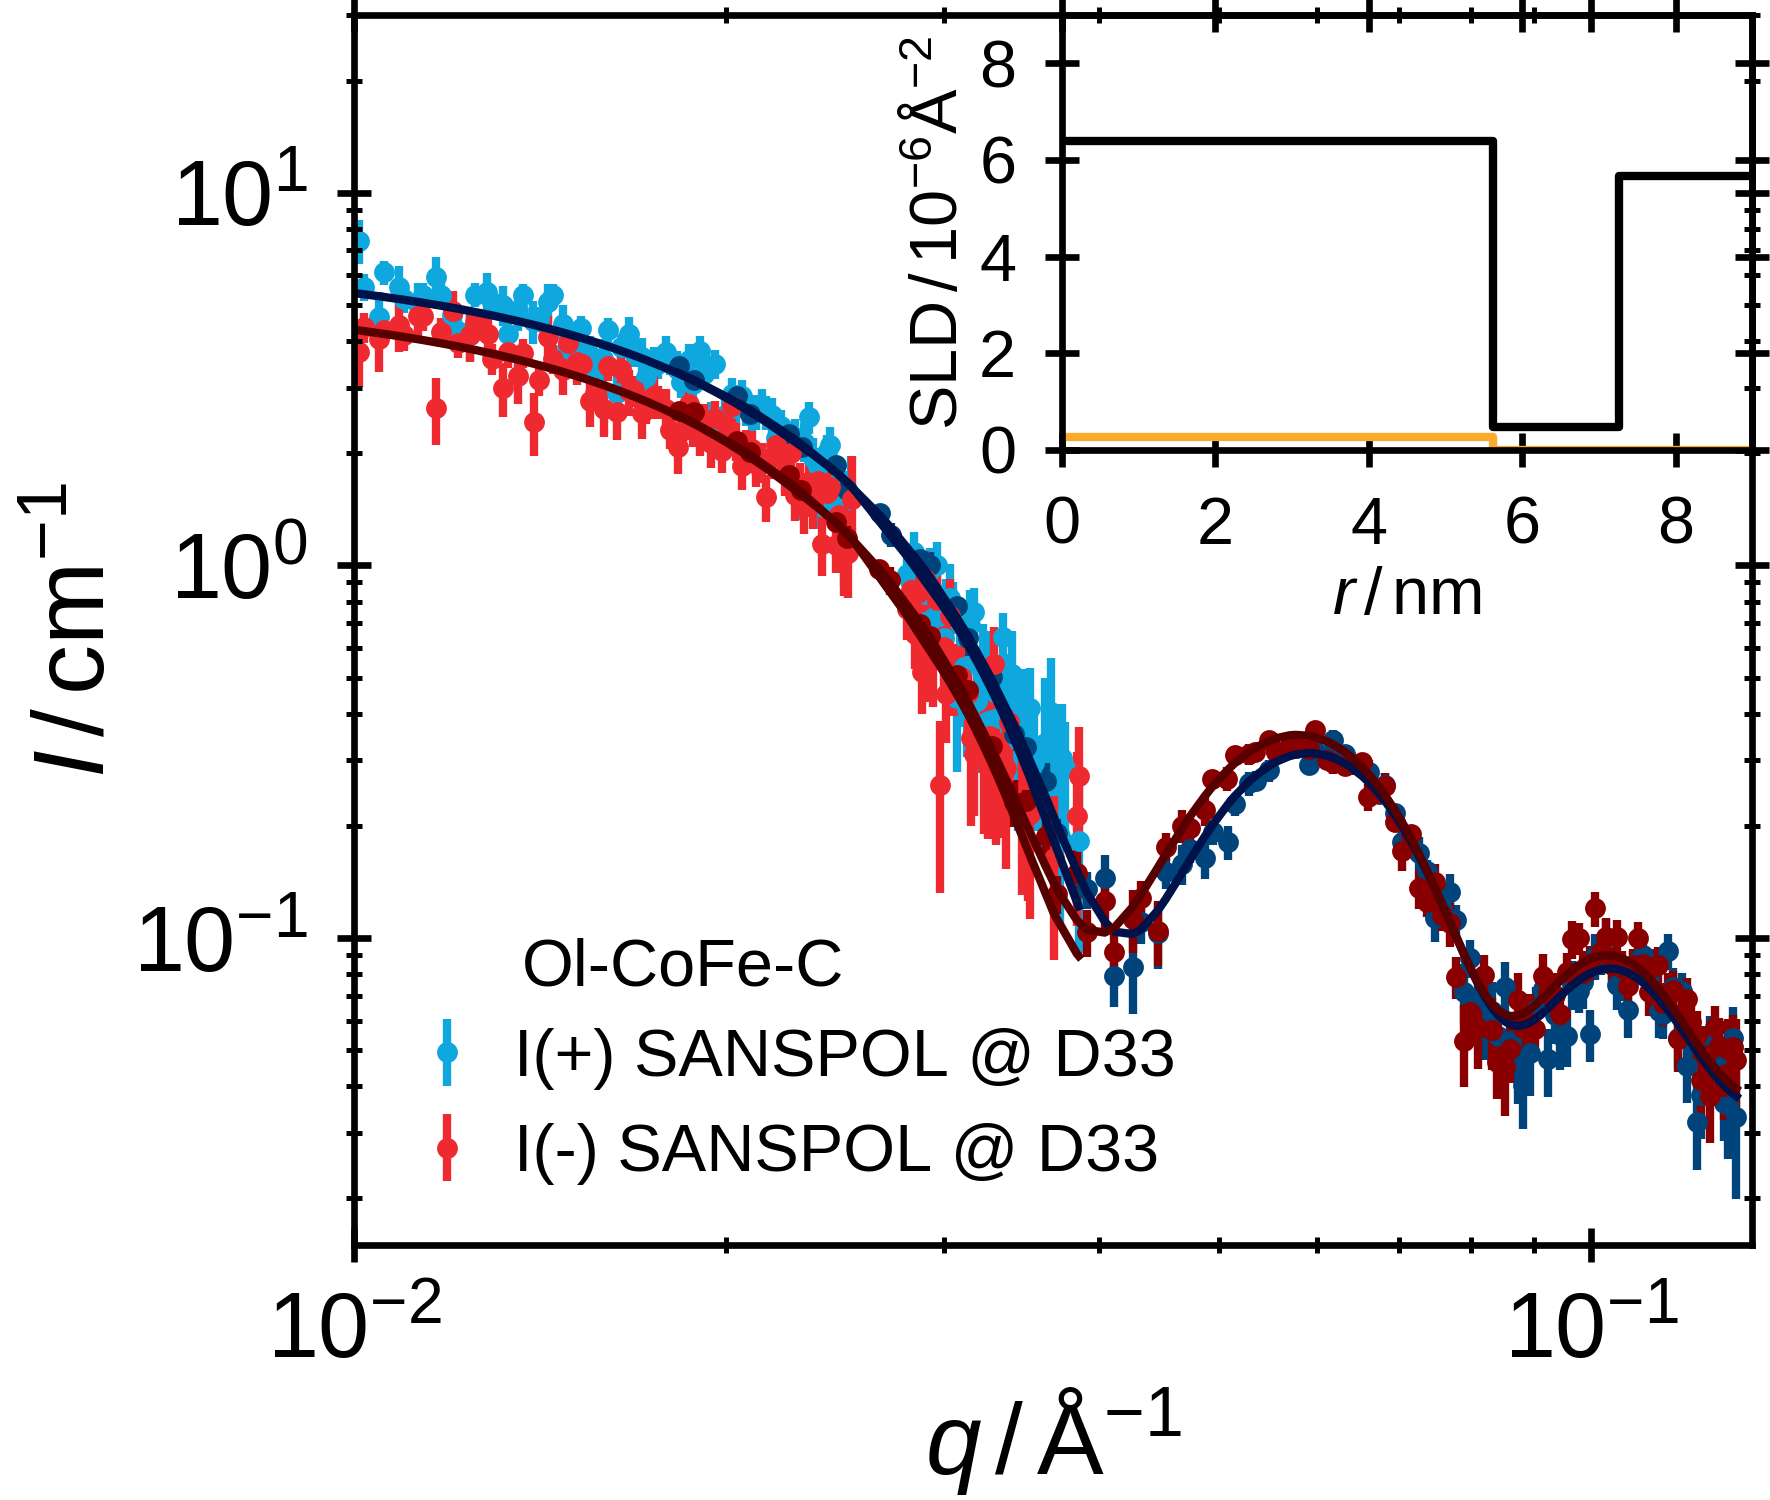
\includegraphics{monolayers_SAS_Ol_CoFe_C_SANSPOLFit}
      \caption{\label{fig:monolayers:nanoparticle:sas:OlCoFeC}SAXS and SANS data of Ol-CoFe-C fit to a superball form factor with a background of oleic acid micelles (left). The inset shows the electron SLD and the nuclear SLD of the superball. Additionally, the resulting magnetic scattering length density profile of Ol-CoFe-C by fitting the SANSPOL data obtained at $1.2 \unit{T}$ is shown (right).}
    \end{figure}

    \reffig{fig:monolayers:nanoparticle:sas:OlCoFeC} shows the experimental SAS data for Ol-CoFe-C.
    The measured form factors present better defined minima than the acetylacetonates nanoparticles and the third form factor maxima is recognizable in both SAXS and SANS, which is a sign for a small size-distribution.
    The SAXS and SANS data of Ol-CoFe-C are fit simultaneously with a core-shell superball of variable core-shell SLD to self-consistently determine the nanoparticle core-shell structure and composition.
    The thereby determined form factor shown in \reffig{fig:monolayers:nanoparticle:sas:OlCoFeC} describes both data sets in good agreement and is described by the parameters tabulated in \reftab{tab:monolayers:nanoparticle:sans:superballOlFit}.

    The shell is hereby determined to have a composition of \ch{Co_{0.82} Fe_{2.18} O_4} and the core \ch{Fe_{0.48(1)} Co_{0.52(1)} O}.
    The formula units are constrained in the fitting process with the iron to cobalt ratio obtained for the particles from EDX $N_{\ch{Fe}} / N_{\ch{Co}} \eq 2.49$ and the volumes of the inverse spinell and w\"ustite phases.
    This yields a particle core radius of $1.7 \unit{nm}$ and a shell thickness of $3.4 \unit{nm}$.
    The fitted size distribution of $6.2 \%$ is a log-normal distribution for the combined core and shell thickness $R \eq r_\mathrm{core} + d_\mathrm{shell}$ instead of only the core or shell, which provides better conditions in the fitting process and is directly comparable to size distributions measured from TEM.
    Additionally, a size distribution for the spinel shell $d_\mathrm{shell}$ is varied separately and obtained as $18(4) \%$ with a relatively large uncertainty.

  \paragraphNewLine{Comparison of SAS with TEM and XRD}
    To compare the sizes by the best superball fits obtained with SAS to the sizes determined by TEM and XRD, they are listed in \reftab{tab:monolayers:nanoparticle:saxs:sizeComparison}.
    For Ac-CoFe-C and Ol-CoFe-C, the sizes obtained from SAXS and TEM are in a similar order of magnitude and deviate less than $10 \%$ from each other.
    For Ac-CoFe-C-2 the deviation is larger and especially the obtained size distribution is of greater magnitude in SAXS in contrast to TEM.
    Possibly, the evaluated TEM micrographs covered a too small specimen size and therefore the obtained size and size distribution do not reflect the true averaged sizes of the nanoparticle batch.

    The comparison with XRD reveals that for both cases of Ac-CoFe-C the obtained crystallite sizes are smaller than the SAXS results.
    This hints to lattice disorder in the nanoparticle volume, which results in a smaller coherent crystalline grain size than the morphological particle size.
    This can be given by structural disordered towards the particle surface.

    \begin{table}[!htbp]
      \centering
      \caption{\label{tab:monolayers:nanoparticle:saxs:sizeComparison}Comparison of nanoparticle length scales as viewed by small-angle scattering, electron microscopy and X-ray diffraction.}
      \begin{tabular}{ c | l | l | l }
                            & \textbf{SAS} & \textbf{TEM} & \textbf{XRD}\\
        \hline
        \multicolumn{4}{l}{\textbf{Ac-CoFe-C}}\\
        \hline
        $a \, / \unit{nm}$  & $9.38(2)$       & $10.1(1)$ & $5.285(3)$\\
        $\sigma_a \, / \%$  & $11.9(1)$       & $13.9(9)$ & \\
        \hline
        \multicolumn{4}{l}{\textbf{Ac-CoFe-C-2}}\\
        \hline
        $a \, / \unit{nm}$  & $8.58(8)$       & $10.8(1)$ & $5.916(5)$\\
        $\sigma_a \, / \%$  & $15.0(4)$       & $9.9(8)$  & \\
        \hline
        \multicolumn{4}{l}{\textbf{Ac-CoFe-C-3}}\\
        \hline
        $a \, / \unit{nm}$  & $11.38(4)$       & $12.5(1)$ & \\
        $\sigma_a \, / \%$  & $11.0(1)$        & $13.2(9)$ & \\
        \hline
        \multicolumn{4}{l}{\textbf{Ol-CoFe-C}}\\
        \hline
        $a_\mathrm{core} \, / \unit{nm}$      & $3.4(2)$        &           & $9.767(3)$\\
        $d_\mathrm{shell} \, / \unit{nm}$     & $3.4(1)$        &           & $3.124(1)$\\
        $a_\mathrm{total} \, / \unit{nm}$     & $10.2(2)$       & $10.9(1)$ & \\
        $\sigma_{a, total} \, / \%$           & $6.2(3)$        & $8.8(3)$  & \\
        $\sigma_{d} \, / \%$                  & $18(4)$         &           & \\
        \hline
      \end{tabular}
    \end{table}

  \paragraphNewLine{Magnetic Properties from SANSPOL}
    Fixing the structural result from SAS, the nanocubes Ac-CoFe-C, Ac-CoFe-C-2 and Ol-CoFe-C have additionally been measured with polarized neutrons at a strong magnetic field to determine the particle magnetization.
    For the single-phased nanocubes Ac-CoFe-C and Ac-CoFe-C-2 a single parameter for the magnetic SLD of the nanocubes if sufficient to explain the observed magnetic splitting at $1.2 \unit{T}$ shown in \reffig{fig:monolayers:nanoparticle:sanspol:superballAcAcFit}.
    The parameter corresponds to $334(5) \unit{kA \, m^{-1}}$ and $444(3) \unit{kA \, m^{-1}}$ for Ac-CoFe-C and Ac-CoFe-C-2, respectively.
    In comparison to the bulk magnetization of cobalt ferrite of $450 \unit{kA \, m^{-1}}$ \cite{Tachiki_1960_Origi}, the observed particle magnetization of Ac-CoFe-C-2 is remarkably close, and Ac-CoFe-C reaches $75 \%$ of the bulk value.
    The reduced value could originate from the lower cobalt to iron ratio in the sample.

    For the core-shell nanocubes Ol-CoFe-C shown in \reffig{fig:monolayers:nanoparticle:sas:OlCoFeC}, the simultaneous refinement of the core and shell magnetization yields that the complete magnetization is given by the shell, and no magnetic contribution is found from the nanoparticle core.
    This connects well to the assumption that the nanocubes consist of a core in a w\"ustite phase and a shell in an inverse spinell phase, and that the particles are not actually fully oxidized with anti-phase boundaries throughout the nanoparticle volume.
    The shell magnetization is relatively weak with $113(12) \unit{kA \, m^{-1}}$, which indicates that the shell might not be perfectly crystallized in a single inverse spinell phase, but possibly anti-phase boundaries are still present.
    Averaging the shell magnetization over the complete particle volume, an average particle magnetization of $109(13) \unit{kA\, m^{-1}}$ is observed.
\end{document}